%% Das Layout des Dokumentes wird festgelegt. Hier A4 mit einer 10er Schrift. Typ: Report 
\documentclass[a4paper,10pt,oneside]{article}

\usepackage[ngerman]{babel}
\usepackage[utf8]{inputenc}
\usepackage[T1]{fontenc}
\usepackage{amsmath}
\usepackage{graphicx} 
\usepackage{a4wide}

%%Wenn ein Absatz nicht eingerückt werden soll
\setlength{\parindent}{0em}
 
%%Abstand zwischen Absätzen
\setlength{\parskip}{2.0ex plus 1.0ex minus 0.5ex}
 
%% das war der Vorspann, in dem die Formatierungsregeln festgelegt werden
 
%%Nun kommt das Dokument:
 
%%Anfang
\begin{document}

\tableofcontents
 
\section{fickerboy}
Hier steht der Inhalt.
hören und sehen du ficker
äöü

\section{11 - HMM (Hidden Markov Models)}
	\begin{itemize}
		\item Modellieren Sequenz von Datenpunkten
		\item benötigen zugrundeliegendes state modeling
		\item oft zusammen mit GMMs verwendet
	\end{itemize}
	
\subsection{Sequenzmodellierung und State-Modelierung}
	\begin{itemize}
		\item Sequenzmodellierung ist in typischer Signalverarbeitungskette letzte Schritt nach Datenverarbeitung und State Modeling 
		\item Klassifikation und Sequenzmodellierung eng miteinander verbunden
	\end{itemize}

\subsection{Dynamic Time Warping}
	\begin{itemize}
		\item einfaches Verfahren zum Vergleich von Sequenzen
		\item Algorithmen in der HMM-Modellierung sehr ähnlich zu DTW
		\item Wir haben: Aufnahmen von Sprachsignalen - Trainingsdaten (Beispielaufnahmen mit bekanntem Inhalt) + Testdaten (Aufnahmen mit unbekanntem Inhalt)
		\item Ziel: Wir wollen die Distanz einer unbekannten Sequenz und einer Beispielsequenz berechnen
		\item Frame für Frame-Vergleich Probleme: Signale sind unterschiedlich lang + Anfang und Ende der Äußerung nicht bekannt
		\item Faggot-Lösung: Lineares Alignment - für fast alle Zwecke aber viel zu unflexibel
		\item Killer-Lösung: DTW
				\begin{itemize}	
					\item basiert auf Prinzip des dynamischen Programmierens (DP) bzw. der minimalen Editierdistanz
					\item Pfade durch eine Matrix von möglichen Zuordnungen berechnet
					\item Ergebnis: Distanzmaß zwischen den beiden Äußerungen
				\end{itemize}
	
		\item Ziel: Finde Distanz zwischen den beiden Äußerungen (je niedriger desto besser)
		\item Problem: Alle Pfade müssen betrachtet werden um den Besten zu finden
		\item Lösung:
				\begin{itemize}
					\item Berechne für jede Zeit $t$ die kumulativen Distanzen $\alpha(s,t)$, die die Distanz der Teiläußerungen bis zu den Zuständen q(s,t) (s=,1,..,S)  beschreiben
					\item Die Distanzen für Zeitpunkt t+1 berechnen sich iterativ aus denen für Zeitpunkt t und hier wird Minimierung der Distanz durchgeführt
				\end{itemize}
					\item Benötige Distanzmaß $d(s,t)$ für den beobachteten Frame t und den Referenzframe s (z.B. euklidische Distanz)
 		\end{itemize}
 		\centering
 		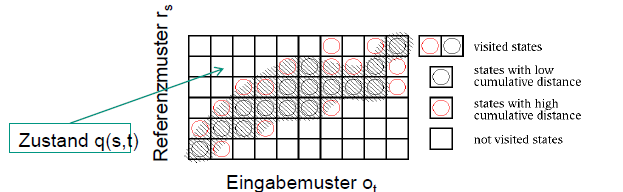
\includegraphics[scale=0.65]{Grafiken/DTW_Beispiel.png}
 		
 		\begin{itemize}
 			\item Welche Übergänge zwischen Frames sind möglich? Was haben sie für Distanz-Kosten?
 			\item Erlaubt sind überlicherweise:
 				\begin{itemize}
 					\item Ersetzung: Kosten = d(.,.) (praktisch immer > 0)
 					\item Einfügung/Auslassung eines Frames: Kosten können in der Praxis ignoriert werden
 					\item Einfügung/Auslassung mehrerer Frames: evtl. Extra-penalty, max. Zahl von Frames, die ausgelassen werden dürfen
 				\end{itemize}
 		\end{itemize}
\vspace{5px}
\flushleft Ablauf des Algorithmus:
 			\begin{itemize}
 				\item Initialisierung: Beginne bei Startzustand $q(0,0)$, $t:=0$, $\alpha(0,0):=d(0,0), \alpha(x,0)=\infty$
 				\item Für jeden Zustand $q(s,t)$:
 					\begin{itemize}
 						\item Betrachte jeden erlaubten Zustandsübergang $q(s',t-1) -> q(s,t)$
 						\item Finde min. Distanz zu $q(s,t)$
 						\item Bis Teildistanz $\alpha(s,t)$ einen gewissen Grenzwert überschreitet
 					\end{itemize}
 				\item weitere Einschränkungen des Suchraums denkbar
 				\item Komponenten der Zustandsmatrix Schritt für Schritt berechenbar (zeiteffizient + speichereffizient)
 			\end{itemize}
 		\begin{itemize}
 			\item Anwendung in der Spracherkennung
 			\item z.B. heute noch praktisch bei der Erkennung von sehr kleinen Vokabularen
		\end{itemize} 	
		
\vspace{5px}
\flushleft Probleme bei Unterscheidung einer kleinen Menge von Wörtern:
		\begin{itemize}
			\item benötigt eine Endpunktdetektion
			\item wird sehr ineffizient wenn viele Trainingsbeispiele vorhanden sind - großes Vok. braucht extrem viele Trainingsbeispiele
			\item Trainingsdaten können nicht zwischen verschiedenen Referenzen geteilt werden
			\item Erkennung unbekannter Wörter ist nicht möglich
			\item ungeeignet für kontinuierliche Sprache
			\item sehr kurze Wörter sind schwer zu trainieren
		\end{itemize}
	$\Rightarrow$ Andere Methode wird benötigt die es ermöglicht, kleinere Einheiten (Silben, Phoneme) zu trainieren und zu erkennen 		

\subsection{Markov-Modelle}
Sprachproduktion als stochastischer Prozess
	\begin{itemize}
		\item Beobachtungen zur Sprachproduktion:
		\begin{itemize}
			\item das gleiche Wort/Phonem hört sich jedesmal anders an
			\item in einem gegebenen Zustand können verschiedene Laute mit 		unterschiedlicher Wahrscheinlichkeit beobachtet werden
			\item der Produktionsprozess kann Übergänge aus einem Zustand in einen anderen machen, aber nicht alle denkbaren Übergänge sind möglich, zumindest nicht gleich wahrscheinlich
		\end{itemize}
		\item Sprachprozess befindet sich zu jedem Zeitpunkt in einem Zustand
		\item In jedem Zustand werden Laute ausgegeben entsprechend einer gewissen Wahrscheinlichkeit: Emissionswahrscheinlichkeit
		\item Die Übergänge zwischen Zuständen erfolgen auch entsprechend einer gewissen Wahrscheinlichkeitsverteilung: Übergangs- oder Transitionswahrscheinlichkeiten
		\item Markov-Modelle:
			\begin{itemize}
				\item Es gibt eine diskrete Zustandsmenge ${s_1, ... ,s_N}$
				\item Wir beobachten eine probabilistische Zustandssequenz $O = (o_1,...,o_T), o_i \in  {1,...,N}$
				\item Markov-Annahme: Wahrscheinlich, dass wir zum Zeitpunkt t in einem gewissen Zustand sind, hängt nur von vorhergehendem Zustand ab
				\item Verteilung soll stationär (zeitunabhängig) sein
			\end{itemize}
	\end{itemize}
	
\subsection{Hidden-Markov-Modelle}
Markov-Modelle und Spracherkennung
	\begin{itemize}
		\item Zustand $<=>$ Beobachtung
		\item In der Sprache haben wir aber ein Kontinuum an möglichen Tokens (typischerweise Sprachsignalframes), die endlich vielen Zuständen (Phonemen) zugeordnet werden sollen
		\item In der Sprache sind die Zustände versteckt (hidden)
	\end{itemize}
	
Hidden-Markov-Modelle (HMM) 
	\begin{itemize}
		\item sind ein doppelter stochastischer Prozess
			\begin{itemize}
				\item Zustandsabfolge probabilistisch
				\item Jeder Zustand emittiert seine Beobachtung: Diese Emission ist ebenfalls probabilistisch
				\item Zustandsfolge ist versteck (hidden)
			\end{itemize}
		\item Sind Markov-Modelle (1. Ordnung)
			\begin{itemize}
				\item Wahrscheinlichkeiten für den Eintritt in den nächsten Zustand hängen nur vom aktuellen Zustand ab
			\end{itemize}
		\item Nichtbeobachtbarkeit der Zustandsfolge hat eine Reihe von Konsequenzen		
			\begin{itemize}
				\item Sprachdekodierung mit HMMs: Anhand der Beobachtungen auf eine mögliche Zustandssequenz rückschließen (dabei wird man nie die exakte Lösung erhalten, sondern nur eine mit höchster Wahrscheinlichkeit)
				\item Training von HMMs: Kennen zwar die durchlaufene Zustandsfolge, aber nicht die Zeitpunkte der Zustandsübergänge
			\end{itemize}
			\centering 
			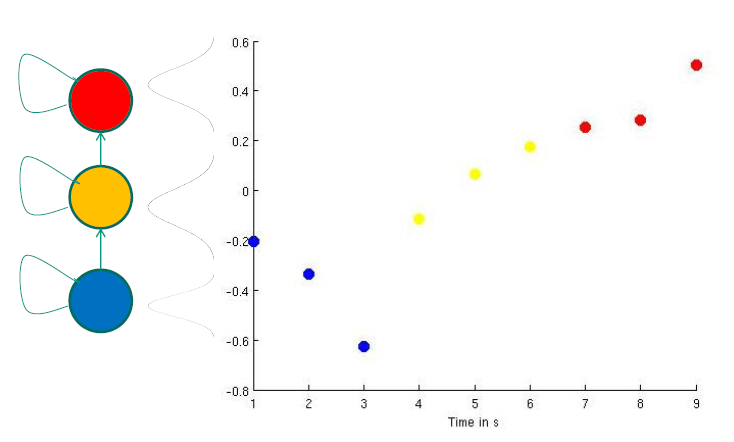
\includegraphics[scale=0.5]{Grafiken/hmm-darstellung.png}
	\end{itemize}

Formale Definition:
	\begin{itemize}
		\item HMM $\lambda = (S,\pi, A,B,V)$
		\item $S={s_1,...,s_N}$ - Menge aller möglichen Zustände
		\item $\pi$: $\pi(s_i) = P(q_1 = s_i)$ - Anfangsverteilung bei t=1
		\item $A=((a_{ij})), 1 \leq i, j \leq n$ - Matrix von Übergangswahrscheinlichkeiten
	\end{itemize}
 		
 		
 		
 		
 		
 		
 		
 		
 		
 		
 		
 		
 		
 		
 		
 		
 		
 		
 		
 		
 		
 		
 		
 		
 		
 		
 		
 		
 		
 		
 		
 		
 		
 		
 		
 		
 	

 
%%Ende
\end{document}